\documentclass{pgnotes}

\title{Mid-size data centre environments}

\begin{document}

\maketitle

\section{Data hall}

The data hall is the main area of interest in a data centre where IT equipment is housed, \autoref{fig:data-hall-schematic}.
Data centre environments may have one or more data halls, sometimes called suites.

\begin{figure}[htbp]
  \centering
  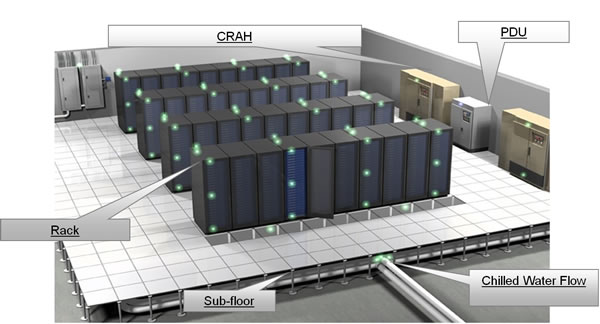
\includegraphics[width=1.0\linewidth]{data_hall}
  \caption{Data hall schematic (TSM tutorials)}
  \label{fig:data-hall-schematic}
\end{figure}

\subsection{Raised floor}

The data hall often has a raised floor, meaning that the tiles can be removed and a space exists under the floor, \autoref{fig:raised-floor}.
It is somewhat similar to a false-ceiling in reverse.

\begin{figure}[htbp]
  \centering
  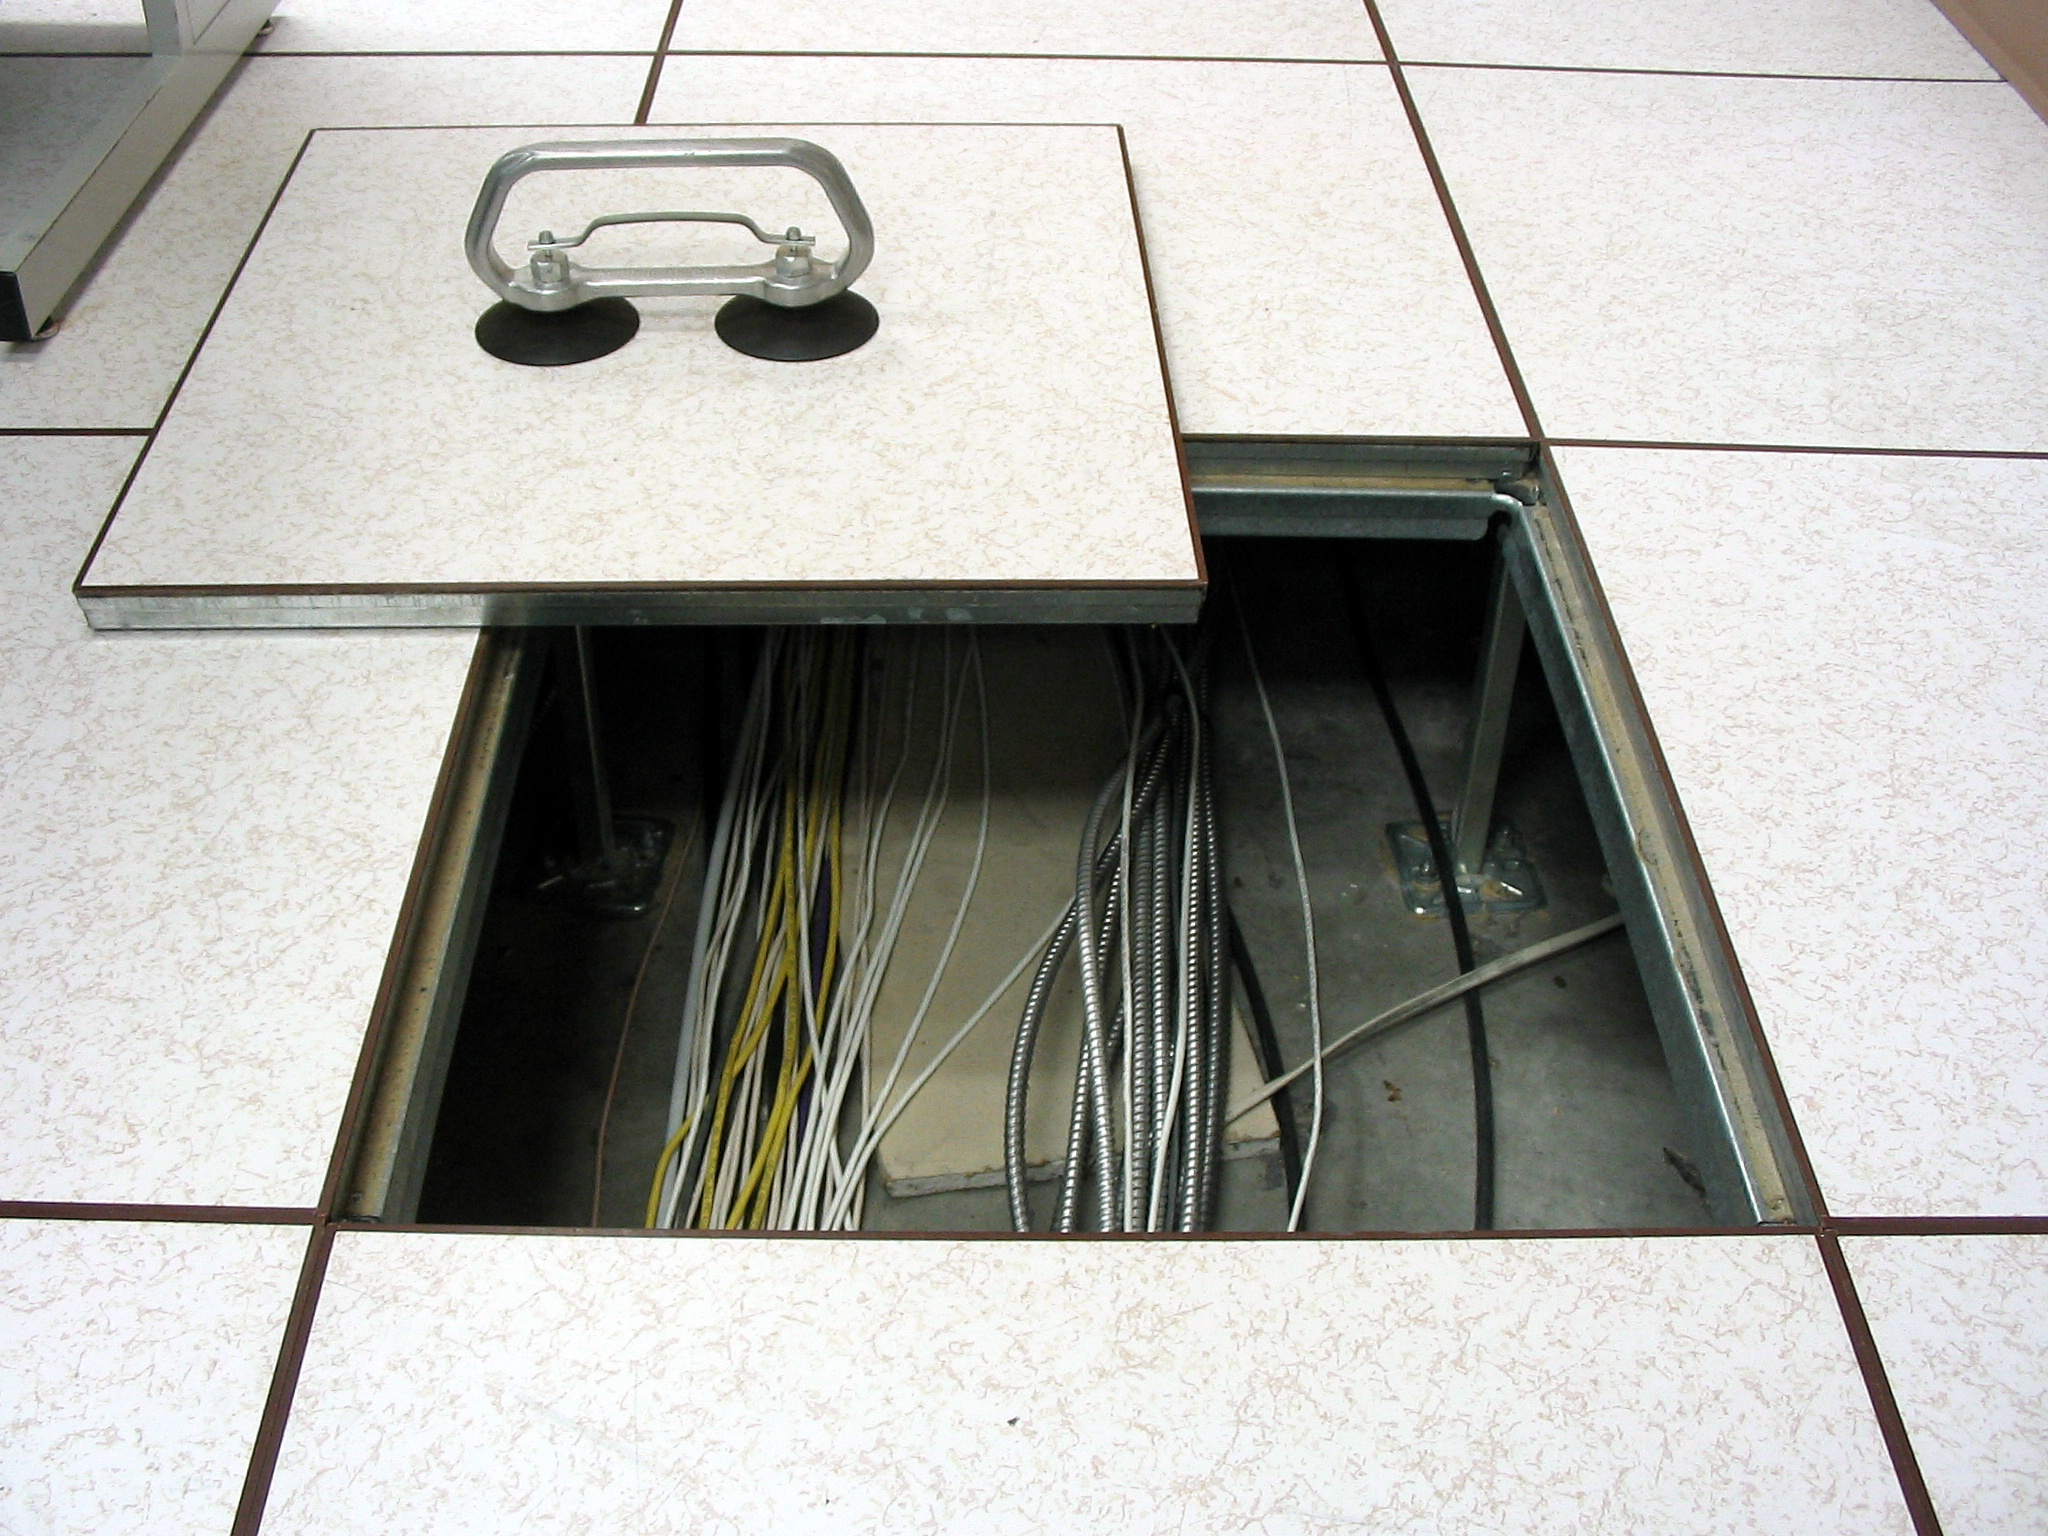
\includegraphics[width=0.75\linewidth]{raised_floor_wikipedia}
  \caption{Raised floor (Wikipedia)}
  \label{fig:raised-floor}
\end{figure}

Not all data centres have raised floors.
Where present, the raised floor has two key functions:
\begin{itemize}
\item Provides space for cooling air to circulate. Some times are solid but others are perforated to allow air to escape. More on that later.
\item Allows cables to be routed and re-routed easily. 
\end{itemize}

\subsection{Cage}

A cage is a subdivision of a data hall to demarcate a number of racks for security or regulatory purposes.

\begin{figure}[htbp]
  \centering
  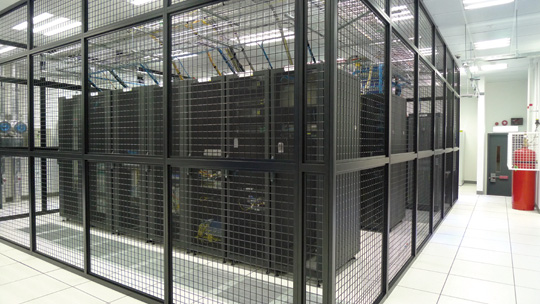
\includegraphics[width=1.0\linewidth]{cage}
  \caption{Cage (Equinix)}
  \label{fig:cage}
\end{figure}


\subsection{Rows}

Where more than one cabinet is required, they are normally placed beside each other to form a row.
The number of cabinets in a row will depend on spatial and usage requirements.

\subsection{Aisle}

An aisle is where two rows of cabinets face each other.
Data centres normally use a hot aisle/cold aisle arrangement where servers face each other front-on or rear-on.
This is to aid in cooling (see later).

\begin{figure}[htbp]
  \centering
  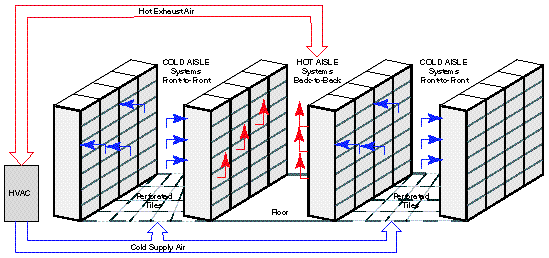
\includegraphics[width=1.0\linewidth]{hot_cold_aisle_oracle}
  \caption{Hot/cold aisle (Oracle)}
  \label{fig:hot-cold-aisle}
\end{figure}

\end{document}

